
\section{Discussion}
\label{sec:discussion}

In this section, we discuss the physical implications of our empirical
findings regarding bow shock shapes.  Our most reliable result is the
average shape of the OB bow shocks from the 227 MIPSGAL sources with
quality rating of 3~stars or higher.  This yields mean values of
\(\Pi = 1.78 \pm 0.06\) and \(\Lambda = 1.72 \pm 0.02\), or median values of
\(\Pi = 1.57\) and \(\Lambda = 1.69\).  The uncertainty quoted on the mean
values is the ``standard error of the mean'':
\(\text{sem} = \sigma / \sqrt{n}\), where \(\sigma\) is the rms dispersion and
\(n\) is the number of sources.  Note that in the case of the
planitude \(\text{sem}(\Pi) = 0.06\) is considerably smaller than
\(\text{mean}(\Pi) - \text{median}(\Pi) = 0.21\), so the latter would be a
more conservative estimate of the uncertainty.\footnote{This is
  because the distribution of \(\Pi\) is approximately log-normal, which
  yields a significant tail towards high values when converted to
  linear space.}  These values can be compared with the predictions of
the thin-shell wilkinoid model \citep{Wilkin:1996a}, which are
\(\Pi = 1.67\), \(\Lambda = 1.73\) when the bow shock axis lies in the plane
of the sky (following Paper~0, this is defined as the zero point of
the inclination angle, \(i\)).  When the axis is inclined, both
planitude and alatude are predicted to decrease but not by very much,
tending to \(\Pi = 1.5\), \(\Lambda = 1.63\) as
\(\abs{i} \to \ang{90}\) (see \S~5.3 of Paper~0).  The median observed
value\footnote{In the presence of outliers, the median is a more
  robust estimate of the central tendency than is the mean.} falls
squarely inside this range for both the planitude and alatude, which
is a remarkable triumph for the \citet{Wilkin:1996a} model.

On the other hand, turning now to the \emph{variety} of bow shock
shapes, we see that the wilkinoid can no longer explain our results.
The rms dispersions of the planitude and alatude distributions for the
MIPSGAL sources are \(\sigma(\Pi) = 0.87\) and
\(\sigma(\Lambda) = 0.30\) (Tab.~\ref{tab:big-p}), which are respectively 5 times
and 3 times larger than the total range of variation of \(\Pi\) and
\(\Lambda\) predicted for the wilkinoid surface.  Although some of the
dispersion is due to uncertainties in the observations and the fitting
algorithm, this contribution is expected to be small, especially for
the larger, well-resolved sources, for which systematic uncertainties
in the methods for determining \(\Pi\) and \(\Lambda\) will
dominate. Conservative upper limits to the relative size of these
uncertainties were estimated in \S~7 of Paper~0 to be \(< 20\%\) for
\(\Pi\) and \(< 10\%\) for \(\Lambda\), whereas the observed dispersions are
roughly twice as large: \(\sigma(\Pi)/\Pi = 55\%\) and
\(\sigma(\Lambda)/\Lambda = 18\%\).  Furthermore, the variations in planitude and
alatude are readily apparent by eye, as is demonstrated by the example
bow shock images shown in Figure~\ref{fig:mipsgal-shapes}b.  Sources
such as K123 have very typical shapes and fall near the center of the
\(\Pi\)--\(\Lambda\) distribution, whereas high-\(\Pi\) sources such as K447 have
a very flat apex region, while low-\(\Pi\) sources such as K566 have a
pointier, almost triangular apex.  High-\(\Lambda\) sources, such as K517,
have very open wings that bend away from the star, while
low-\(\Lambda\) sources such as K489 have closed wings and a semi-circular
appearance.


In Paper~0 we found that certain bow shock shapes can show a much
greater variation in their projected appearance as a function of
inclination angle than is seen for the wilkinoid.  For example, the
cantoids and ancantoids, which have asymptotically hyperbolic far
wings, can shift towards higher apparent planitude and alatude as the
inclination increases, generally with \(\Lambda \ge \Pi\) (Fig.~20 of Paper~0).
This might plausibly explain the vertical spur towards higher
\(\Lambda\) seen in the empirical distribution (\S~\ref{sec:ob-shapes}). A
different behavior is shown by bow shocks with very flat apex regions,
such as the MHD simulation from \citet{Meyer:2017a} that is analyzed
in the \S~6 of Paper~0.  This shows a high planitude \(\Pi\) when the
orientation is exactly edge-on, but \(\Pi\) decreases sharply along a
roughly horizontal track as the inclination \(\abs{i}\) increases
(Fig.~25 of Paper~0).  This is similar to the principal axis of
variation of the observed shapes (e.g.,
Fig.~\ref{fig:mipsgal-shapes}a).

If such variations in orientation do make a significant contribution
to the observed distribution of bow shock shapes in the
\(\Pi\)-\(\Lambda\) plane, then various predictions follow, which might be
observationally tested.  High-planitude sources with \(\Pi > 3\) would
be expected to have low inclinations, \(\abs{i} < \ang{30}\), whereas
high-alatude sources with \(\Lambda > 2\) would be expected to have high
inclinations, \(\abs{i} > \ang{45}\).  Unfortunately, determination of
the inclination for individual sources requires high resolution
spectroscopy of emission lines in order to map the kinematics of the
flow in the bow shock shell \citep[e.g.,][]{Henney:2013a}.  This is
not currently available for the majority of the MIPSGAL sources, which
are detected only by their dust continuum emission.  A further
prediction for the high-alatude sources is that the environmental flow
should be divergent rather than plane-parallel, in order to give a
cantoid shape instead of a wilkinoid.  This would tend to favor
``weather-vane'' cases, where the interstellar medium is flowing past
the star, and disfavor ``runaway'' cases, where the star is moving
through a static medium.  However, in \S~\ref{sec:corr-shape} we found
no significant difference in the shape distributions as a function of
the bow shock environment.  Figure~\ref{fig:mipsgal-uncorrelated}a
shows that the alatudes of sources that are facing \hii{} regions or
\SI{8}{\um} bright-rimmed clouds (and therefore might be expected to
be immersed in a champagne flow) are no higher than sources that are
isolated.


\begin{figure}
  (a)\\
  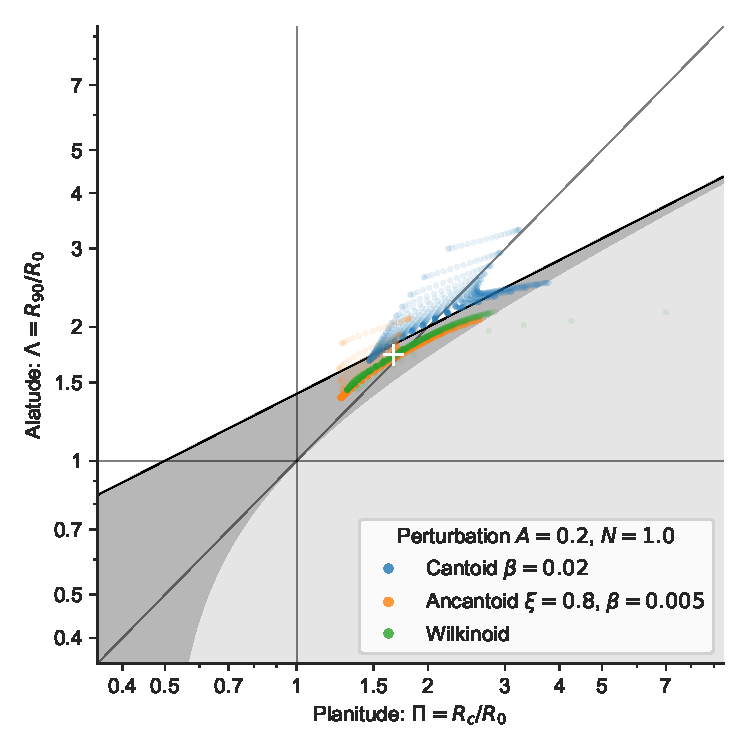
\includegraphics[width=\linewidth]
  {figs/wave-R90-vs-Rc-A020-N10}
  (b)\\
  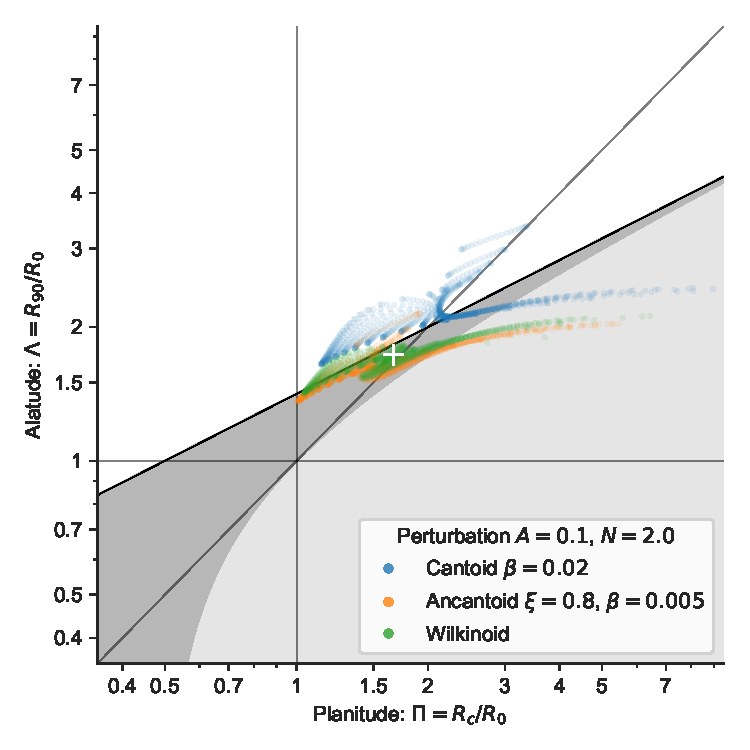
\includegraphics[width=\linewidth]
  {figs/wave-R90-vs-Rc-A010-N20}
  \caption{Diagnostic diagram for perturbed shapes from standing wave
    oscillations.  Each model is characterized by a base shape
    (colored symbols, as described in key) and an amplitude, \(A\),
    and wavenumber, \(N\), of the oscillation: (a)~breathing mode with
    \(N = 1\), \(A = 0.2\); (b)~curling mode with \(N = 2\),
    \(A = 0.1\) (see Fig.~\ref{fig:perturb-shapes} for the
    phase-dependent intrinsic shapes).  The plotted points show the
    varying planitude and alatude of the projected bow shock shapes
    with uniform sampling over an entire period of the oscillation and
    for varying inclinations (sampled according to an isotropic
    distribution of orientations).  Each individual point is plotted
    with a low opacity so that the crowding of points in certain
    regions of the plane can be appreciated.}
  \label{fig:perturb-Rc-R90}
\end{figure}

An alternative explanation for the variety of observed bow shock
shapes is that they are due to time-dependent perturbations to an
underlying base shape.  For instance, multiple studies have shown that
stellar bow shock shells can be unstable \citep{Dgani:1996a,
  Dgani:1996b, Blondin:1998a, Comeron:1998a, Meyer:2014a}, leading to
large amplitude oscillations in the shell shape.  The oscillations are
found to be most vigorous when the post shock cooling is highly
efficient, allowing the formation of a thin shell (see Paper~I).  Even
in cases where the shell is stable, oscillations may be driven by
periodic variations in the stellar wind mass-loss rate or velocity, or
by inhomogeneities in the ambient stream.  Rather than using a
particular dynamical model of these oscillations, we instead crudely
simulate their effect by assuming a constant amplitude standing wave
perturbation to the base shape, as described in
Appendix~\ref{sec:perturbed-bows}.  Example results are shown in
Figure~\ref{fig:perturb-Rc-R90} for an ensemble of bows with different
orientations and phases of oscillation, considering three different
underlying base shapes.  It can be seen that modest amplitudes of 10
to 20\% can give rise to a distribution in \(\Pi\) and \(\Lambda\) similar to
that observed for the MIPSGAL sources when the oscillation wavelength
is of same order as the bow shock size.

An attractive feature of the oscillation hypothesis is that it
naturally explains why we find little correlation between the bow
shock shape and other source parameters (\S~\ref{sec:corr-shape}).
The one significant correlation that we do find is that the alatude
distribution is broader for bow shocks with larger angular sizes.
This might be explained if the relative amplitude of oscillations were
higher for sources with more powerful winds.  However, in that case it
is hard to understand why no such variation is seen in the width of
the planitude distribution.

We now address the difference in shape distribution between the
different classes of source.  Compared with the OB star bow shocks,
the cool star sample from \citet{Cox:2012a} shows a significantly
smaller alatude of \(\Lambda = 1.41 \pm 0.03\) (see
Fig.~\ref{fig:herschel-compare-mipsgal}).\footnote{Although the
  planitude also appears to be slightly smaller, this is not very
  statistically significant due to the small number of cool star
  sources and the large width of the OB star planitude distribution.}
Such a closed shape for the wings is inconsistent with the wilkinoid
value of \(\Lambda = \text{\numrange{1.63}{1.73}}\), which is surprising
given that the emission shells in these sources are relatively narrow
(Figs.~\ref{fig:herschel-arc-fits}
and~\ref{fig:herschel-arc-fits-poor}), so one might have thought that
the thin-shell approximation of \citet{Wilkin:1996a} would be
\emph{more} appropriate than for the OB stars, but this is clearly not
the case.  One possible explanation for this 



%%% Local Variables:
%%% mode: latex
%%% TeX-master: "obs-bowshocks"
%%% End:
